%************************************************
\chapter[Appendix 3.4: Chapter 3 - Connectance and interaction ratio]{Appendix 3.4: Chapter 3 - Network assembly, connectance, and interaction type ratio}\label{ch:Appendix3.4}
%************************************************
\renewcommand{\thefigure}{A.3.4.\arabic{figure}}
\setcounter{figure}{0}

\renewcommand{\thetable}{A.3.4.\arabic{table}}
\setcounter{table}{0}

Any set of interaction rules that prevents a pair of species from interacting modifies the connectance of the interaction network by an adjustment on the number of potentially feasible links. Connectance measured relative to a fully-connected network only makes sense if every pairwise interaction is potentially feasible. Otherwise, connectance should be computed relative to the potential number of links given the assembly contraints of the network. Linkage rules will vary among interaction types, so that in a multi-interaction network the potential number of links will be different for each sub-network.

Hence, specifying type-specific connectances and linkage rules, the probability that a given link is of a certain type can be obtained. For the sake of brevity, we name this set of probabilities the Interaction Type Ratio (ITR henceforth, where if a subscript is given, it indicates the probability of a certain interaction type). In the following example we demonstrate the difference between assuming a single value of connectance and setting type-specific connectances for network assembly, given the linkage probabilities of \cref{fig:fig3.1}. These linkage probabilities can be summarised qualitatively in that for commensalism and mutualism, every pairwise link is allowed, while amensalism can only occur between species of the same trophic level, antagonism does not occur in a bottom-up fashion (i.e. where the species from the lower level benefits to the expense of a species of an upper level), and competition only occurs between species of the same or adjacent levels.

Assume a network with $N = 20$ nodes. If no link is structurally forbidden when we consider the overall network, the potential number of links is:

\[S = N(N-1)/2 = 190\]

Furthermore, imposing an overall connectance \(C = 0.2\) and equal ITR, i.e. \(ITR_x = 0.2\) for every interaction type \(x\), yields the following number of realised links:

\[L = C*S = 38, L_x \approx 8\]

With these numbers, we may calculate the specific connectances of every interaction type for this particular network. Take as an example a community generated with the constraints and parameterization stated in chapter 3 and in Appendix 3.1 (e.g. four discrete trophic levels, abundance scaling across trophic levels, 2000 individuals at the basal trophic level). The linkage rules can be expressed mathematically to obtain the number of potential links per interaction type. The scaling constraints predict that, on average, the distribution of the \(N\) species in the \(T = 4\) trophic levels will be \(\{N_1 = 7, N_2 = 6, N_3 = 4,N_4 = 3\}\). Then:

\begin{align*}
& S_{amensalism} = \sum_{i = 1}^T {N_{i}(N_i-1) \over 2} = 49 \\
& S_{antagonism} = N(N-1)/2 = 190 \\
& S_{commensalism} = N(N-1)/2 = 190 \\
& S_{competition} = \sum_{i = 1}^T {N_{i}(N_i-1) \over 2} + \sum_{j = 1}^{T-1} N_j*N_{j-1}= 123 \\
& S_{mutualism} = N(N-1)/2 = 190
\end{align*}


Hence, the type-specific connectances are:

\begin{align*}
& C_{amensalism} = L_{amensalism}/S_{amensalism} = 0.163 \\
& C_{antagonism} = L_{antagonism}/S_{antagonism} = 0.042 \\
& C_{commensalism} = L_{commensalism}/S_{commensalism} = 0.042 \\
& C_{competition} = L_{competition}/S_{competition} = 0.065 \\
& C_{mutualism} = L_{mutualism}/S_{mutualism} = 0.042 \\
\end{align*}

By definition, type-specific connectances will be lower than the overall connectance. Only in the unrealistic scenario of networks with a single interaction type, its specific connectance will equal the overall connectance, while all the other types will have a specific connectance of zero. As overall connectance increases, more links are realised for each interaction type, and type-specific connectances will increase in turn. Fig. \ref{fig:figApp3.4.1} shows the variation in type-specific connectances as overall connectance increases for networks in which interactions are realised with equal probability for each interaction type.

\begin{figure}[!ht]
\centering
\includegraphics[width=\textwidth]{./Figures/Appendix3_4/Fig_1.png}
\caption[Connectance and interaction frequencies]{\color{Gray} relationship between overall connectance and a) specific connectances of each type, b) ITR. Black line in panel a) shows the y=x line}
\label{fig:figApp3.4.1}
\end{figure}

Note how the ratio between type-specific connectance and overall connectance varies with the type of interaction. This is a direct consequence of the linkage rules that define the set of potential links available to each interaction type: smaller sets of potential links necessarily yield higher connectances for the same number of realised links. Also, given the set of linkage rules chosen, it is not possible to obtain networks of \(ITR_x = 0.2 , \forall x\) and overall connectance on the range of \(C \geq 0.6\). In this case, this is due to the fact that amensalistic interactions occurr only between species of the same trophic level, and assuming that any two species cannot interact in more than one way, these links can potentially be `filled' by any other interaction type.Therefore, an upper limit to the amensalistic realised interactions is imposed not only by its ITR, but also by the occurrence of other interaction types. Once this limit is reached for amensalistic interactions, other interaction types, however, still maintain part of their potential link space unoccupied, and therefore can keep increasing in number of links, connectance and, hence, ITR.

If, instead of imposing a constant ITR, we assemble networks with fixed specific connectances, the overall connectance and ITR will vary accordingly. As in the example above, assume a network with \(N = 20\) nodes, the same linkage rules and, therefore, same potential number of links per interaction type. In this case, setting \(C_x = 0.2 \forall x\) yields the following approximate number of links:

\begin{align*}
& L_{amensalism} = C_{amensalism} * S_{amensalism} = 9 \\
& L_{antagonism} = C_{antagonism} * S_{antagonism} = 38 \\
& L_{commensalism} = C_{commensalism} * S_{commensalism} = 38 \\
& L_{competition} = C_{competition} * S_{competition} = 25 \\
& L_{mutualism} = C_{mutualism} * S_{mutualism} = 38
\end{align*}

\[L = \sum_x L_x = 148\]

and ITR:

\begin{align*}
& ITR_{amensalism} = L_{amensalism}/L = 0.06 \\
& ITR_{antagonism} = L_{antagonism}/L = 0.257 \\
& ITR_{commensalism} = L_{commensalism}/L = 0.257 \\
& ITR_{competition} = L_{competition}/L = 0.166 \\
& ITR_{mutualism} = L_{mutualism}/L = 0.257
\end{align*}

Not surprisingly, ITRs are not equivalent to specific connectances, given that the potential link set is different for each interaction type. The value of overall connectance for this network is:

\[C = \frac{\sum_x L_x}{S} = 0.78\]

As specific connectance values increase, overall connectance quickly reaches 1 (Fig. \ref{fig:figApp3.4.2}). Once this threshold is crossed, increases in specific connectance are no longer reflected in the assembled network, and in fact, an increasing number of links cannot be realised. Therefore, assuming that most interactions are allowed (i.e. not structurally forbidden), as in the linkage rules used here, specific connectances as low as \(\approx 0.25\) for every interaction type already fill the entire set of potential links. These numbers apply to binary connectances, that consider only the presence or absence of a given interaction. If quantitative interactions are available, weighted connectances can be obtained, and these will better reflect the effective number of links \citep{Ulanowicz2014a}.

\begin{figure}[!ht]
\centering
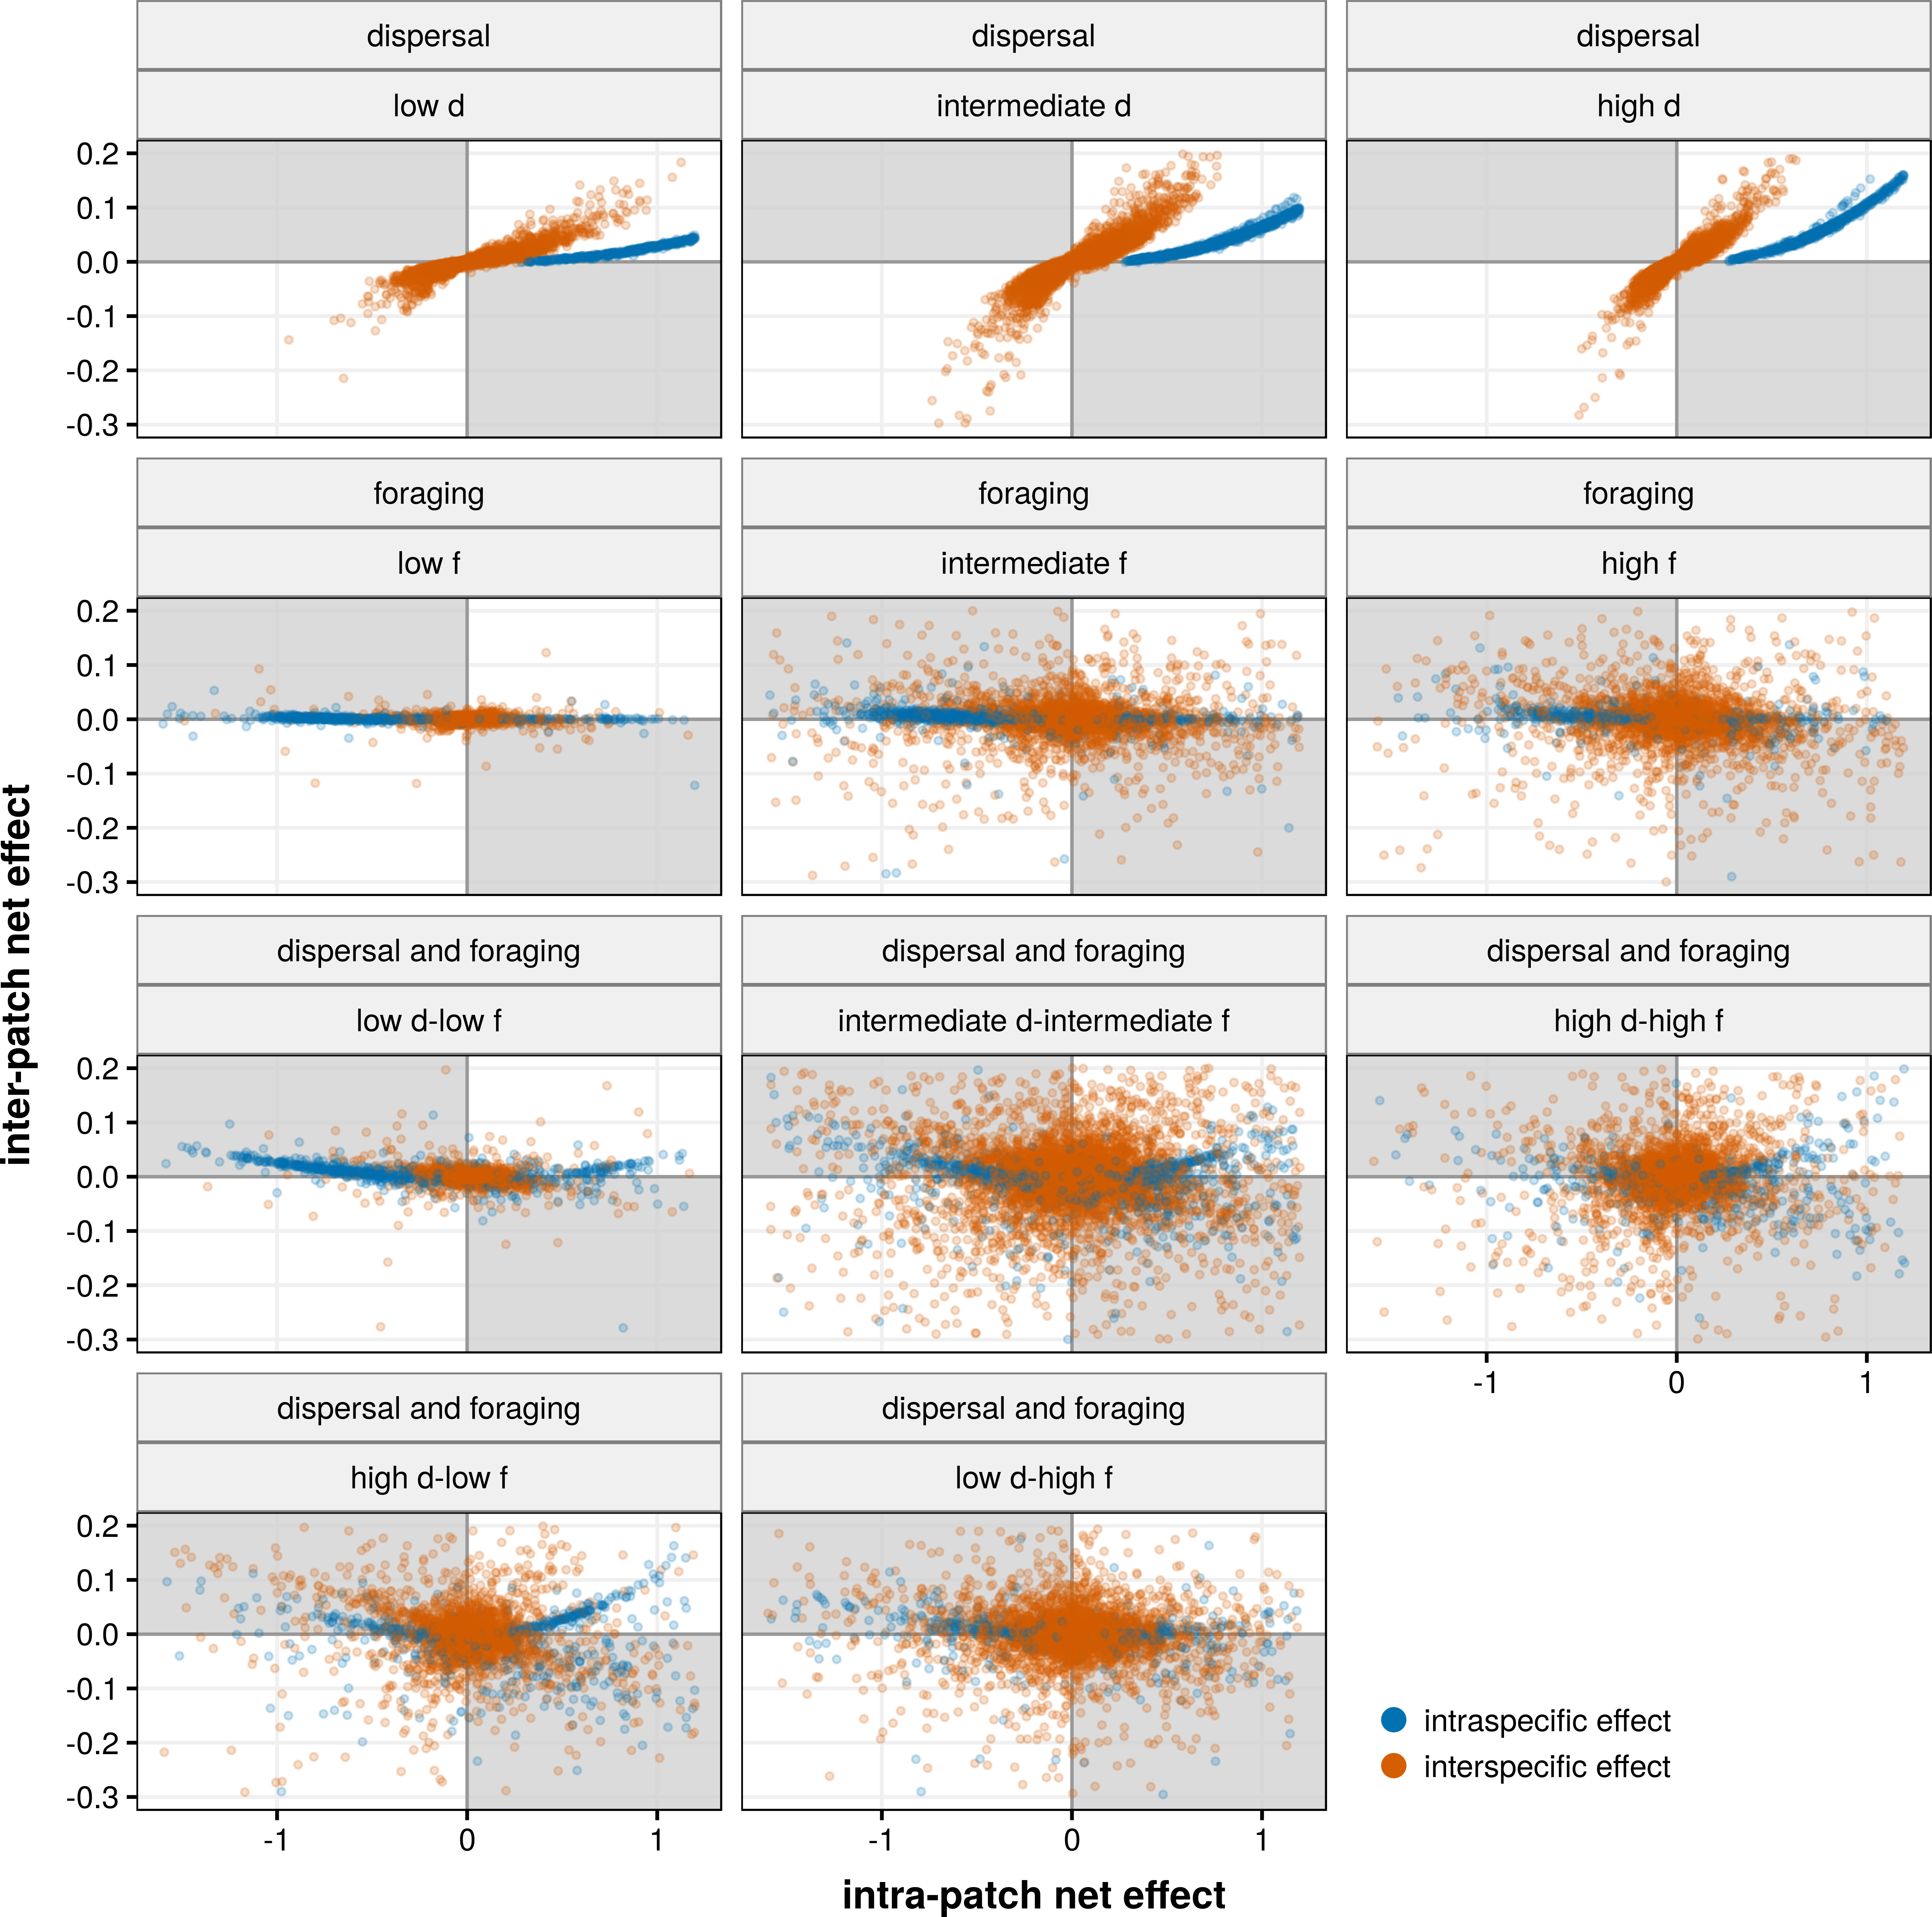
\includegraphics[width=.5\textwidth]{./Figures/Appendix3_4/Fig_2.png}
\caption[Overall and specific-type connectances]{\color{Gray} relationship between specific connectances and overall connectance, assuming equal specific connectances for each interaction type. Black line shows the y=x line. Note that axes are switched with respect to Fig. \ref{fig:figApp3.4.1}, for reflecting the behaviour of the overall connectance.}
\label{fig:figApp3.4.2}
\end{figure}
